\documentclass[11pt]{article}
\usepackage[margin=1in]{geometry}
\usepackage[T1]{fontenc}
\usepackage{lmodern}
\usepackage{amsmath,amssymb}
\usepackage{booktabs}
\usepackage{graphicx}
\usepackage[numbers,sort&compress]{natbib}
\usepackage[colorlinks=true,linkcolor=blue!50!black,citecolor=blue!50!black,urlcolor=blue!50!black]{hyperref}
\usepackage{xcolor}
\usepackage{enumitem}
\setlist{itemsep=2pt,topsep=4pt}

\title{Compile or Learn? Weight-Space Programming versus Fine-Tuning,\\and Why to Combine Them}
\author{Puneet Bajaj}
\date{}

\begin{document}
\maketitle

\begin{abstract}
A capable language model can now change a smaller model by reading its weights and editing them directly, with no gradients. This \emph{weight-space programming} promises small, readable, cheap fixes. Before anyone uses it in place of fine-tuning, two questions need answers: for which problems does it work, and what does an edit do to the rest of the model?

We compare it with LoRA fine-tuning in a controlled study. The model, answer format, forward-pass budget and the programmer's written brief are held fixed. The tasks are chosen to differ mainly in how much of the needed knowledge the model already has, measured with a linear probe, though they also differ in format and data. Four tasks run from ``present'' to ``absent'': SST-5 sentiment, SST-5 with mirrored labels, real people's survey answers, and facts about invented people. Twenty programmer runs, eighteen of them independently audited and one excluded for breaking the no-fitting rule, cover two programmer models and two base-model families (Qwen2.5-1.5B and SmolLM2-1.7B).

Three regimes emerge.
\begin{itemize}
  \item \textbf{Redirect.} When the model knows the answer but reads it out wrongly, every programmer found the same two-row embedding swap. It matched LoRA, and was more reliable than LoRA's default configuration: default LoRA learned the mirrored task on only one of three seeds, and needed three times the data to learn it on all three.
  \item \textbf{Compile.} When the answer is a table, programmers compiled the labels into hand-built circuits that recall 900 invented facts perfectly. Those circuits bypass the network and reduce MMLU to chance, on both model families. Edits written through the model's own pathways score lower but keep it intact.
  \item \textbf{Learn.} When the improvement needs a better input-to-answer mapping, LoRA wins, even when trained on only 256 examples.
\end{itemize}

Two findings change how the method should be used:
\begin{itemize}
  \item \textbf{The brief decides the edit type.} Told to preserve the model, a programmer switched from a destructive circuit to an intact edit.
  \item \textbf{The methods are complements, not rivals.} Fine-tuning on top of a programmed edit reaches 99.0--99.7\% on facts with a tenth of the training presentations LoRA alone needs. On the mirrored task it learns on every seed of both model families (56--59\%), where LoRA alone needs three times the data to do the same; a hand-written version of the swap works as well as the programmer's edit. The edit saves training data rather than raising the ceiling, and the combined models keep general ability.
\end{itemize}
In our runs, weight-space programming behaved like a compiler: a fast way to write rules and tables into a model, judged by what else it changes, and a starting point that cuts the data gradient training needs.
\end{abstract}

\section{Introduction}

Today, changing what a neural network does almost always means training it. You collect examples, run gradient descent, and get back a change spread across millions of parameters that nobody can read. A recent line of work offers a different route. A capable language model, the \emph{programmer}, reads another network's weights, runs a handful of forward passes, works out how the computation goes, and writes the change directly into the weights~\citep{takehi2026sparks}. In the original demonstration, the programmer removed one direction from 131,072 weights in two MLP layers of Qwen3.5-0.8B. That stopped the model looping on maths problems and raised MATH-500 accuracy from 7.9\% to 48.1\%. No gradients were involved, and the fix could be read and checked. Follow-up work has applied the idea to larger language models, biosignal classifiers and game-playing networks~\citep{hu2026exploring,varam2026mixed,lehmann2026compiling}.

If this \emph{weight-space programming} (WSP) worked broadly, it would change how models are patched. Edits could be small enough to review, cheap in GPU time, and built from a few thousand labelled examples rather than a training run. But most evidence so far reports what programming achieved, not how it compares with the obvious alternative; the one direct comparison covers a single published patch on one task family~\citep{yang2026writing}. Someone holding a pretrained model that misbehaves needs to decide whether to program it or fine-tune it. That decision turns on two questions:
\begin{enumerate}
  \item \textbf{When does programming work, compared with fine-tuning?} The repair above rearranged knowledge the model already had. Can a programmer also add knowledge the model lacks? And where it can, how does it compare with gradient training on the same task and the same model?
  \item \textbf{What does an edit cost?} An edit that fixes the target task might break everything else, and measuring only the target task would never show it.
\end{enumerate}

\paragraph{How we test it.} We built a comparison in which one factor varies: how much of the needed knowledge the base model already has. Four five-option tasks span the range:
\begin{itemize}
  \item \textbf{SST-5 sentiment}~\citep{socher2013sst}. The model knows this and reads it out correctly, though imperfectly.
  \item \textbf{SST-5 inverted.} The same prompts with mirrored labels. The model knows the sentiment but reads it out backwards.
  \item \textbf{Twin-2K}~\citep{toubia2025twin}. Predicting a real person's survey answer. The model knows what people in general tend to say, but little about individuals.
  \item \textbf{Fictional facts.} Questions about 300 invented people, with no context. The model cannot know these.
\end{itemize}
A linear probe on the base model's activations measures how much of each answer is already there. Everything else is held fixed: the model, the answer format, the budget of 50 forward passes, and a written brief that every programmer receives. Each programmer is an independent Claude agent, and an independent auditor checks every run afterwards. The baseline is LoRA~\citep{hu2022lora}. The main model is Qwen2.5-1.5B-Instruct~\citep{qwen2025}. We repeat the key experiments on SmolLM2-1.7B-Instruct, a different model family.

\paragraph{What we expected, and what happened.} We expected programming to work in proportion to what the model already knows: good at redirecting, unable to add. The first half held.
\begin{itemize}
  \item \textbf{Mirrored labels: every programmer found the same fix.} All five programmers who attempted the task, across two programmer models and both base models, swapped the embeddings of `` negative'' and `` positive''. A control swap of two unrelated words did nothing.
  \item \textbf{The swap matched LoRA, and was more reliable than its default configuration.} Default LoRA failed to learn the task on two of three seeds.
\end{itemize}
The second half did not hold.
\begin{itemize}
  \item \textbf{Programmers added knowledge by compiling it.} Faced with facts the model could not know, they turned the training labels into explicit lookup circuits that recalled every fact under unseen wordings. On survey answers, a similar circuit beat LoRA.
  \item \textbf{Those circuits break the model.} After them, the model scores at chance on MMLU and almost never predicts the next token of ordinary text (0--0.1\% top-1, against 46\%). This held on both model families (Figure~\ref{fig:tradeoff}).
  \item \textbf{Through edits mostly keep the model intact.} An edit that stored the facts through the model's own memory pathway recalled fewer of them (77\%), but left the model as capable as before, just as LoRA does.
\end{itemize}

\begin{figure}[t]
\centering
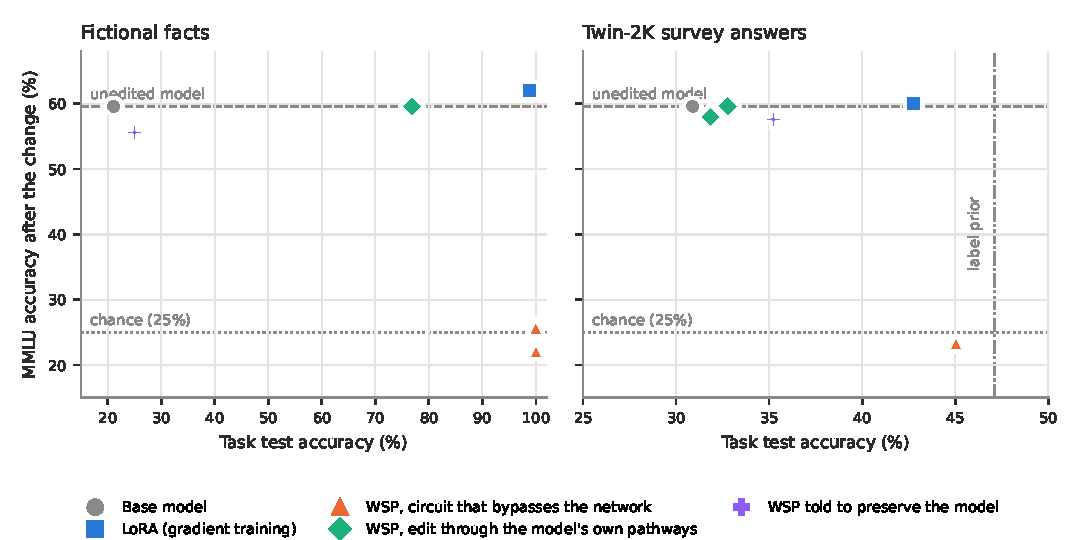
\includegraphics[width=\linewidth]{figures/tradeoff.pdf}
\caption{The trade-off behind the best weight-space programming results (Qwen2.5-1.5B). Each point is one way of teaching the model a task it cannot already do. Horizontal axis: test accuracy on that task. Vertical axis: the model's MMLU accuracy afterwards. Circuits that bypass the network (orange) reach the highest task accuracy and leave the model at chance on MMLU. Edits through the model's own pathways (green), edits from a programmer told to preserve the model (purple) and LoRA (blue) keep MMLU near the unedited level.}
\label{fig:tradeoff}
\end{figure}

\paragraph{Two follow-up experiments changed the picture.}
\begin{itemize}
  \item \textbf{Telling the programmer to preserve the model changes the edit it builds.} The brief said nothing about side effects, so we added a requirement to preserve the model's other abilities. On survey answers, the same programmer then switched from a destructive circuit to a gated edit that gains 4.3 points and leaves the model's other abilities unchanged. On facts, it could not find an edit that both added knowledge and passed the preserve check.
  \item \textbf{Programming and fine-tuning combine.} Running LoRA on top of a programmed edit raised facts accuracy to 99.0--99.7\% with 4,000 training examples. LoRA alone needed about ten times as much data. On mirrored labels the combination reached 57--59\%, well above either method alone.
\end{itemize}

\paragraph{So what.} For anyone deciding how to change a model, the results give a usable map:
\begin{itemize}
  \item \textbf{Redirect.} When the model has the knowledge but uses it wrongly, program it. The fixes are tiny, readable and reproducible, and more reliable than default fine-tuning.
  \item \textbf{Compile.} When the answer is a table that can be written from the labels, programming matches or beats fine-tuning. But its most accurate route disables the model, so the edit must be checked, and the brief must ask for preservation.
  \item \textbf{Learn.} When the improvement needs a better mapping from inputs to answers, fine-tune.
  \item \textbf{Combine.} In both regimes where we tried it, a programmed edit was a good starting point for fine-tuning, and the combined models kept general ability.
\end{itemize}
For anyone evaluating edits, target-task accuracy is not enough. The highest-scoring edits are the most damaging. Raw perplexity misleads in the opposite direction: it flags harmless temperature changes as damage. We propose a small side-effect protocol that avoids both traps.

\paragraph{Contributions.}
\begin{enumerate}
  \item A controlled comparison of weight-space programming with gradient fine-tuning on pretrained language models that varies how much the model already knows, with 20 independent programmer runs across two programmer models and two model families. Every edit and log is released, and every run that produced an edit, apart from an early pilot, is independently audited.
  \item A map of three regimes (redirect, compile, learn), with independent replications. That includes a fix five programmers found separately and three different SST-5 mechanisms that hit the same ceiling.
  \item Evidence that the most accurate programmed edits bypass the network and destroy general ability, on both model families. Edits through the model's pathways do not, and an instruction to preserve the model moves the programmer from one kind to the other.
  \item Evidence that programming and fine-tuning are complementary: a programmed edit fixes both LoRA failure modes we observed, slow storage of new facts and a stuck start on a confidently wrong task. The combined models keep general ability.
  \item An evaluation protocol for weight-space programming: a fixed brief, a ledgered budget, independent audits, and side-effect measures that a temperature change cannot fake.
\end{enumerate}

\section{Background and related work}

Weight-space programming sits between two older ways of changing a model. Knowledge editing writes specific facts into the weights with closed-form updates. Fine-tuning changes behaviour broadly through gradient descent. Our question is which of the two programming behaves like, and when.

\paragraph{Weight-space programming.} \citet{takehi2026sparks} introduced the setting. A frontier model, the \emph{programmer}, gets read and write access to a network's weights and a small budget of forward passes, and must change its behaviour without gradient descent. Their experiments range from identifying a network's training data from its weights, to writing small policy networks from scratch, to repairing Qwen3.5-0.8B's reasoning loops by ablating one direction in the MLPs of layers 15 and 19. Notably, the same programmer could not improve Gemma~3 270M, a model that rarely looped. That is an early hint that programming works best where a specific failure exists to be fixed.

\paragraph{Follow-up work.} Several studies have since extended the idea:
\begin{itemize}
  \item \citet{hu2026exploring} ran 16 editing trajectories on Qwen3.5-0.8B and 9B, with embeddings, final norm and output head frozen.
  \begin{itemize}
    \item They found large, localised gains on some benchmarks, mostly from suppressing failure behaviours such as reasoning loops, and no validated improvement in 6 of 16 trajectories.
    \item Their cross-task tests found mostly positive transfer, with some unquantified regressions.
    \item Gains were largest where the base model was weakest.
  \end{itemize}
  \item \citet{varam2026mixed} report that programmers can write biosignal classifiers from scratch with far fewer training subjects than gradient descent needs, but cannot improve classifiers that are already well trained.
  \item \citet{lehmann2026compiling} has programmers write game-playing networks from scratch out of a simulator's source code.
  \begin{itemize}
    \item The written weights look like programs, mostly exact zeros and small integers, and beat learners that only see example levels.
    \item They are fragile: weight noise the size of one gradient step removes most of their success, and gradient training cannot improve them.
    \item When asked to repair trained networks, the strongest writers rebuilt them almost entirely, while Claude Opus 5.5 made small edits that never surpassed the original.
  \end{itemize}
  \item \citet{salloum2026treeising} recast the Qwen3.5 repair as discrete optimisation over weight bits, with no language model involved.
  \item \citet{ahmed2026memorization} argue that an LLM's reading of weights relies on local arithmetic plus memorised dataset priors.
  \item \citet{goworek2026replicating} reproduce the original writing and reading experiments and conclude that current writing amounts to compiling hand-designed programs.
\end{itemize}
Closest to our work, \citet{yang2026writing} compare one published patch (the Qwen3.5-0.8B loop repair) with LoRA on spatial reasoning. LoRA reached near-ceiling target accuracy but broke two neighbouring distance tasks that the patch preserved, whether the adapter was trained from the base model or on top of the patch. They conclude that written edits disturb less, and leave broader capability checks and the combination of the two methods open. We differ in four ways:
\begin{itemize}
  \item 20 independent programmer runs under one brief, 18 of them audited, instead of one reused patch;
  \item tasks that vary how much of the needed knowledge the model already has;
  \item general-ability measures (MMLU, next-token accuracy, an unrelated task) alongside the target task;
  \item a test of programming as a starting point for fine-tuning at a matched budget, in the cases where fine-tuning alone fails.
\end{itemize}

Several findings of these follow-up studies line up with ours:
\begin{itemize}
  \item \textbf{Program-like weights.} Lehmann's program-like written weights match what we call compiling. He uses the word for turning known rules into a new network; we use it for writing label-derived tables into an existing pretrained model.
  \item \textbf{Redirection.} Hu et al.'s gains came mostly from suppressing a failure, which is our redirect regime.
  \item \textbf{Already-trained models.} Their failures, and Varam et al.'s, came on models with no identifiable failure or already well trained, which resembles our learn regime.
  \item \textbf{Programmer styles.} Lehmann's contrast between writers who rebuild a network and Opus 5.5's small edits parallels our own split between Fable's bypass circuits and Opus's through edits.
  \item \textbf{Transfer.} Hu et al.'s mostly positive transfer came from small edits to frozen-output models, which is consistent with our finding that edits working through the network leave other abilities intact.
\end{itemize}

\paragraph{Knowledge editing.} ROME~\citep{meng2022rome} and MEMIT~\citep{meng2023memit} locate factual associations in mid-layer MLPs. They insert new associations with closed-form updates, treating the MLP as a key--value store. Those methods compute the update with a solver and, in ROME's case, an optimised value vector. One of our programmers independently built a similar key--value memory from activation statistics alone. Our setting differs in that the programmer must also discover the mechanism and choose where to write, with a small pass budget.

\paragraph{Parameter-efficient fine-tuning.} LoRA~\citep{hu2022lora} trains low-rank updates to the attention and MLP projections and is our gradient baseline. Fine-tuned models need many repetitions to store new facts in a form that survives rephrasing~\citep{allenzhu2023physics}; we see the same effect in our facts task (Section~\ref{sec:compile}).

\paragraph{Probing.} Linear probes~\citep{alain2016probes} measure what information is linearly decodable from a representation. We use a probe at the answer position as a cheap measure of how much of each task's answer the base model already encodes. Section~\ref{sec:discussion} discusses what such a probe misses.

\paragraph{Label remapping.} Models can be asked to answer with flipped or arbitrary labels, and larger models override their semantic priors more easily~\citep{wei2023larger}. Our inverted SST-5 task applies the same idea to a single fixed prompt. The model is never told the labels are mirrored, so any fix has to come from the weights.

\paragraph{Simulating survey respondents.} Twin-2K-500~\citep{toubia2025twin} pairs a large battery of survey answers from 2,058 US respondents with LLM-simulated ``digital twins''. We use it as a task where the needed knowledge is about individuals, which a small model mostly does not have.

\section{Study design}
\label{sec:design}

The aim is a fair comparison between two ways of changing a model: programming its weights and fine-tuning it. One factor varies, how much the model already knows. Every other choice below either holds something fixed or makes the comparison checkable.

\subsection{Models and answer format}
\paragraph{Models.} The main model is Qwen2.5-1.5B-Instruct (28 layers, $d_\text{model}=1536$, tied embeddings) in fp16. It is small enough for free GPUs and large enough to know sentiment and general facts. To check that the findings are not specific to one model, we repeat the key experiments on SmolLM2-1.7B-Instruct (24 layers, $d_\text{model}=2048$, tied embeddings), which comes from a different family and training corpus.

\paragraph{Answer format.} Every task is a chat prompt ending in five options labelled A--E in random order. We score the next-token distribution at the first assistant token, renormalised over the five letters. Because every method optimises the same quantity, they are directly comparable, and the chance level is always 20\%. Because the option order is random, no method can win by learning a favourite letter. We report accuracy with a 2,000-sample bootstrap 95\% interval, and negative log-likelihood (NLL).

\subsection{Four tasks that vary what the model knows}
The tasks step down from ``the model has all the needed knowledge'' to ``it has none'' (Table~\ref{tab:tasks}).
\begin{description}
  \item[SST-5.] Movie-review excerpts from the Stanford Sentiment Treebank~\citep{socher2013sst}, using the original splits: 8,544 train, 1,101 validation (our dev) and 2,210 test. The options are the five sentiment levels.
  \item[SST-5 inverted.] The same prompts and option orders, but the correct answer is the mirrored level: very negative$\leftrightarrow$very positive, negative$\leftrightarrow$positive, neutral unchanged. The prompt never says so. The model has all the knowledge it needs but applies it backwards. This makes it the cleanest test of redirection. It also pairs exactly with SST-5: same inputs, different target.
  \item[Twin-2K.] Each prompt describes one Twin-2K-500 respondent~\citep{toubia2025twin} through 14 demographic answers and 8 of their other survey answers. It then asks a question from the same survey, showing the person's real answer plus four distractors. People are split 1,400 / 200 / 458 into train, dev and test, giving 16,800 / 1,600 / 3,664 examples. A language model knows how people in general tend to answer, but cannot know a particular stranger's answer.
  \item[Fictional facts.] 300 invented people, each with a birth city, profession and hobby (ten possible values per attribute), asked with no context. Any gain must come from information the method itself puts into the weights. All splits ask about the same 900 facts, but with different question wordings: three for train, one for dev and one for test. Credit therefore requires recalling a fact, not reproducing a sentence.
\end{description}

\begin{table}[t]
\centering\scriptsize
\resizebox{\linewidth}{!}{\begin{tabular}{llrrrrrrrr}
\toprule
Task & Knowledge in base model & $n_\text{test}$ & Chance & Prior & Base & Probe & Headroom & \multicolumn{2}{c}{SmolLM2: base / headroom} \\
\midrule
SST-5 & present, read out correctly & 2210 & 19.5 & 23.1 & 44.9 & 47.7 & +5.6 & 36.9 & +1.9 \\
SST-5 inverted & present, read out wrongly & 2210 & 19.5 & 23.1 & 4.0 & 40.8 & +36.1 & 11.4 & +25.0 \\
Twin-2K & population tendencies only & 3664 & 20.4 & 47.1 & 30.9 & 29.2 & -0.9 & -- & -- \\
Fictional facts & absent & 900 & 21.9 & 27.4 & 21.1 & 21.0 & +1.6 & 21.8 & +1.7 \\
\bottomrule
\end{tabular}
}
\caption{The four tasks (test accuracy, \%). \emph{Prior} predicts the most frequent training answer among the options shown: per survey item for Twin-2K, per attribute for facts, and over the whole task for SST-5. \emph{Probe} is the best dev accuracy of a multinomial logistic-regression probe on the base model's residual stream at the answer position. It is read at four depths (a quarter, half, three quarters and all of the layers) and after the final norm, and fitted on 2,048 train examples. \emph{Headroom} is probe minus base accuracy on the probe's dev sample. The last two columns repeat base accuracy and headroom for SmolLM2-1.7B.}
\label{tab:tasks}
\end{table}

\paragraph{Measuring what the model already knows.} A linear probe~\citep{alain2016probes} reads the base model's activations at the answer position and predicts the correct option. If it does much better than the model itself, the model holds information it fails to use, which is exactly what a redirection edit could exploit. Table~\ref{tab:tasks} confirms the intended ordering at both ends, and on both models:
\begin{itemize}
  \item \textbf{SST-5 inverted.} Large headroom: +36 points on Qwen, +25 on SmolLM2.
  \item \textbf{Facts.} None: the probe stays at chance.
  \item \textbf{SST-5.} Small: +6 points on Qwen, +2 on SmolLM2.
  \item \textbf{Twin-2K.} The probe finds nothing beyond the model's own answers. Section~\ref{sec:discussion} explains why this turned out to be incomplete.
\end{itemize}

\subsection{How a programming run works}
Each run is one autonomous Claude agent session working from the same written brief (Appendix~\ref{app:brief}). Runs differ only in a short task description and reference baseline numbers.

\paragraph{What the programmer may do.} It may read any weight and do arithmetic on weight matrices. It has 50 budgeted forward passes over train or dev, each of at most 512 examples, enforced by a persistent ledger. Each pass returns the letter log-probabilities and residual-stream activations at the answer position. It may compute simple statistics of those outputs (means, differences of means, counts, PCA) and write closed-form weight changes it derives itself.

\paragraph{What it may not do.} No gradients, optimisers or LoRA. No regression or classifier solver fitted to labels. No running the network outside the ledger. No reading the test split. These rules stop the programmer from quietly re-implementing fine-tuning. Writing a label-derived table into the weights, such as a list of facts, is allowed but must be disclosed. There is no principled line between ``knowing'' a fact and storing it.

\paragraph{The deliverable.} An edit is a deterministic Python file that changes existing parameter tensors in place; architecture changes are not allowed. The programmer measures its best edit on full dev, and we score every submitted edit on test, which the programmer never sees.

\paragraph{The preserve condition.} The standard brief says nothing about side effects. In a second condition, a short addendum requires the final edit to keep the model's other abilities. The programmer may score the SST-5 dev set (1,101 examples) from the same 50-pass budget, and the edit must keep it at 40\% or above (the base model scores 42.3\%). We also told it that held-out tests of general ability would be run, so it should not tune to the check alone.

\paragraph{Programmers and audits.}
\begin{itemize}
  \item \textbf{Programmers.} Claude Fable 5.2 (runs \texttt{r1}--\texttt{r5}, preserve runs \texttt{p1}, and the SmolLM2 runs \texttt{f1}) and Claude Opus 5.5 (runs \texttt{o1}). One early Twin-2K run, \texttt{r1}, used Fable 5.1 and an earlier brief that discouraged item-level tables; we mark it with an asterisk.
  \item \textbf{Independence.} Runs were independent: each had its own budget and folders, and an instruction not to read other runs' work.
  \item \textbf{Audits.} A separate agent audited every run. The auditor read all of the run's code (for later runs, also the programmer's full transcript), recomputed the reported dev numbers from saved outputs, counted changed weights, checked the ledger against the jobs actually run, and checked for test access and copying.
  \item \textbf{Compute.} Model computation ran only on Kaggle GPUs, never on the programmers' machine.
\end{itemize}

\subsection{The fine-tuning baseline}
LoRA~\citep{hu2022lora} is the standard parameter-efficient fine-tuning method, so it is the natural comparison. We use rank 16, $\alpha=32$, dropout 0.05, all attention and MLP projections, and cross-entropy over the five letter logits. Training uses learning rate $10^{-4}$, an effective batch of 16, and a one-cycle schedule over 4,000 examples (250 optimizer steps).

\paragraph{When the default fails.} We used this default unchanged wherever it worked. On facts it did not learn at all, so we searched until it did and report the working configuration, about fifteen epochs (Section~\ref{sec:compile}).

\paragraph{Extra LoRA experiments.} To make the comparison fair in both directions, we added four:
\begin{itemize}
  \item \textbf{Seeds 1 and 2}, besides seed 0, for both SST-5 tasks.
  \item \textbf{A data learning curve.} Training uses only 256 or 1,024 distinct examples, with the same 250 optimizer steps. This tests whether LoRA's advantage comes from seeing more labels than a programmer, who reads the labels of roughly 2,000--3,000 training examples.
  \item \textbf{LoRA trained on top of a programmed edit}, with the same default configuration and 4,000 examples, over three seeds. This tests whether the methods combine. On SST-5 inverted we also trained it on a hand-written swap of the two label words, and on SmolLM2's edit.
  \item \textbf{Two ways past the SST-5-inverted plateau} for LoRA alone, over three seeds each: a three times larger learning rate ($3\times10^{-4}$), and three times the data (12,000 examples, 750 optimizer steps). This tests whether the edit does anything that tuning LoRA cannot.
\end{itemize}

\subsection{Measuring what an edit costs}
A score on the target task says nothing about what else changed. We use four checks, each catching something the others miss.
\begin{description}
  \item[Option rotation.] For 300 test questions we present all five cyclic rotations of the options. We record how often the model picks the same option text in every rotation. A model that answers by content is consistent; one that leans on position is not.
  \item[Another task.] Each edited model is scored on a different task's dev set: SST-5 for Twin-2K and facts edits (unedited model: 42.3\%), and Twin-2K for SST-5 edits (29.4\%). We skip this for SST-5 inverted, because any successful edit there must invert SST-5 too.
  \item[General knowledge.] Zero-shot MMLU on a fixed sample of 500 questions (unedited Qwen: 59.6\%).
  \item[Language modelling.] We score 200 chunks of 256 tokens from the WikiText-2 test set. We report next-token top-1 accuracy, and NLL after the best single rescaling of all logits.
\end{description}

\paragraph{Why not perplexity?} Many edits include a global temperature change, which fixes overconfidence on the target task. That multiplies every logit by a constant, inflates raw perplexity a hundredfold, and yet leaves every prediction unchanged. Top-1 accuracy is immune to it. The rescaled NLL is fitted on the scored text itself, so it is an upper bound on how much a single temperature can recover.

\paragraph{Controls and statistics.}
\begin{itemize}
  \item \textbf{Controls.} Two edits test whether the SST-5-inverted fix is specific. One swaps two sentiment-unrelated word embeddings (`` table''/`` river''). The other swaps `` negative''/`` positive'' with no other change.
  \item \textbf{Paired bootstrap.} Differences between methods on the same test items are tested with a paired bootstrap (2,000 samples).
  \item \textbf{Temperature-only control.} A temperature fitted on base dev shows how much of an NLL gain a scalar rescale alone could explain.
\end{itemize}

\section{Results}
\label{sec:results}

We take the regimes in order of how much the model already knows. Each subsection asks one question and ends with what it implies. Table~\ref{tab:main} gives every target-task number for Qwen, and Table~\ref{tab:side} gives every side-effect measure.

\begin{table}[p]
\centering\small
\begin{tabular}{llllr}
\toprule
Method & Programmer & Test acc. [95\% CI] & Test NLL & Dev acc. \\
\midrule
\multicolumn{5}{l}{\textit{SST-5}} \\
Base & -- & 44.9 \tiny[42.8, 46.9] & 3.19 & 42.3 \\
Label prior & -- & 23.1 \tiny[21.4, 24.8] & 1.58 & 25.3 \\
LoRA & -- & 59.0 \tiny[57.0, 61.1] & 0.93 & 57.4 \\
WSP r1 & Fable & 47.3 \tiny[45.2, 49.2] & 1.25 & 47.4 \\
WSP r4 & Fable & 48.0 \tiny[45.9, 50.0] & 1.26 & 46.1 \\
WSP r5 & Fable & 46.7 \tiny[44.5, 48.8] & 1.27 & 46.0 \\
WSP o1 & Opus & \multicolumn{3}{l}{no edit beat base} \\
\multicolumn{5}{l}{\textit{SST-5 inverted}} \\
Base & -- & 4.0 \tiny[3.2, 4.8] & 9.59 & 5.0 \\
Label prior & -- & 23.1 \tiny[21.4, 24.8] & 1.58 & 25.3 \\
LoRA & -- & 49.3 \tiny[47.2, 51.4] & 1.08 & 49.8 \\
WSP r1 & Fable & 46.4 \tiny[44.3, 48.5] & 1.26 & 48.1 \\
WSP r2 & Fable & 46.2 \tiny[44.1, 48.3] & 1.26 & 44.2 \\
WSP r3 & Fable & 48.1 \tiny[46.0, 50.1] & 1.23 & 48.4 \\
WSP o1 & Opus & 45.7 \tiny[43.7, 47.7] & 1.24 & 44.8 \\
\multicolumn{5}{l}{\textit{Twin-2K}} \\
Base & -- & 30.9 \tiny[29.4, 32.4] & 2.60 & 29.4 \\
Label prior & -- & 47.1 \tiny[45.4, 48.6] & 1.29 & 47.8 \\
LoRA & -- & 42.8 \tiny[41.2, 44.4] & 1.36 & 40.6 \\
WSP r1 & Fable* & 32.8 \tiny[31.3, 34.2] & 1.51 & 33.2 \\
WSP r2 & Fable & 45.0 \tiny[43.4, 46.6] & 1.38 & 45.8 \\
WSP o1 & Opus & 31.9 \tiny[30.4, 33.3] & 1.52 & 31.7 \\
WSP p1 & Fable, preserve & 35.2 \tiny[33.7, 36.8] & 2.90 & 35.0 \\
\multicolumn{5}{l}{\textit{Fictional facts}} \\
Base & -- & 21.1 \tiny[18.4, 23.7] & 3.46 & 19.4 \\
Label prior & -- & 27.4 \tiny[24.6, 30.4] & 1.59 & 24.1 \\
LoRA & -- & 98.8 \tiny[98.0, 99.4] & 0.10 & 99.2 \\
WSP r1 & Fable & 100.0 \tiny[100.0, 100.0] & 0.00 & 100.0 \\
WSP r2 & Fable & 100.0 \tiny[100.0, 100.0] & 0.01 & 100.0 \\
WSP r4 & Fable & 100.0 \tiny[100.0, 100.0] & 0.00 & 100.0 \\
WSP o1 & Opus & 76.9 \tiny[74.0, 79.4] & 1.03 & 73.0 \\
WSP p1 & Fable, preserve & 25.0 \tiny[22.2, 27.7] & 2.81 & 25.2 \\
\bottomrule
\end{tabular}

\caption{Accuracy (\%) and NLL on Qwen2.5-1.5B. Test accuracy carries a bootstrap 95\% interval. WSP runs \texttt{r}$n$ were programmed by Fable and \texttt{o1} by Opus. \texttt{p1} used the preserve brief. *Twin-2K \texttt{r1} used Fable 5.1 and an earlier brief that discouraged item-level tables; its dev figure is the programmer's own. For runs scored only on test by us, dev is the programmer's full-dev measurement, recomputed by the auditor. LoRA is seed 0; Table~\ref{tab:reliability} gives the other seeds. For facts, LoRA is the fifteen-epoch configuration (Section~\ref{sec:compile}).}
\label{tab:main}
\end{table}

\subsection{Redirect: can programming fix a model that knows but misreads?}
\label{sec:redirect}
SST-5 inverted is built to answer this. The base model scores 4.0\%, far below the 20\% chance level. It is not confused: it confidently picks the true sentiment, which is now always wrong. The probe reads the correct mirrored answer 40.8\% of the time from the same activations, so the knowledge is intact.

\paragraph{Every programmer found the same fix.}
\begin{itemize}
  \item \textbf{Who tried.} Four programmers attempted this task on Qwen (three Fable, one Opus), and one on SmolLM2.
  \item \textbf{What they all did.} Each option line reads ``very negative'', ``negative'', ``neutral'', ``positive'' or ``very positive''. Mirroring the labels is therefore the same as exchanging the words ``negative'' and ``positive''. Each is a single token, so swapping their two rows in the embedding matrix makes every option \emph{read} as its mirror image. The model then does exactly what it did before, matching the review's sentiment to the option text, and lands on the mirrored answer.
  \item \textbf{How much the swap alone does.} It moves dev accuracy from 5.0\% to 44.2--44.3\% in the runs that measured it separately.
  \item \textbf{The finishing touches.} Small additions brought the final Qwen edits to 45.7--48.1\% on test: a temperature rescale against overconfidence, a nudge that lets ``neutral'' be chosen again, and in one run a rank-one intensity correction.
\end{itemize}

\paragraph{The effect is the swap, and it is specific.} Two controls settle this.
\begin{itemize}
  \item Swapping `` negative'' and `` positive'' with no other change scores 46.2\% on test. That is essentially the full Fable \texttt{r1} edit (46.4\%).
  \item Swapping two sentiment-unrelated words (`` table'', `` river'') leaves the model at 4.0\%, exactly where it started.
  \item The same pattern holds on SmolLM2: the swap alone takes it from 11.4\% to 38.6\%, the final edit reaches 45.4\%, and the unrelated swap does nothing (Table~\ref{tab:smollm}).
\end{itemize}

\paragraph{The swap is as good as LoRA and more reliable than its default configuration.}
\begin{itemize}
  \item \textbf{Seed 0: a statistical tie.} LoRA reached 49.3\% with seed 0. The best programmed edit (48.1\%) is not significantly different from it (paired bootstrap, $p=0.37$). The other three are 2.9--3.6 points lower ($p\le0.023$).
  \item \textbf{Other seeds: LoRA mostly fails.} Seeds 1 and 2 never learned the task: 23.9\% and 27.7\% (Table~\ref{tab:reliability}). Training starts confidently wrong (loss 3.9), falls to the uniform-guess plateau ($\ln 5\approx1.61$), and stays there.
  \item \textbf{Seed 0 barely escaped.} It sat on the same plateau for about 200 of its 500 batches. Rerunning it with the same settings as seeds 1--2 reproduced 49.5\%, so the failures are not an artefact of a configuration change.
  \item \textbf{The same failure on SmolLM2.} Its LoRA runs stuck on the same plateau on all three seeds (21.5--22.7\%).
  \item \textbf{More steps get LoRA out; a larger step size does not.} On Qwen, with three times the data (12,000 examples, so three times the steps), all three seeds escaped the plateau between batches 250 and 750 of 1,500 and reached 58.1--61.2\%. With a three times larger learning rate, all three stayed on it (19.4--20.0\%; Table~\ref{tab:plateau}). We tried neither change on SmolLM2.
\end{itemize}
Programming found the fix in every one of its five attempts.

\paragraph{With few labels, programming wins.} With only 256 distinct training examples, LoRA reaches 29.1\% (Table~\ref{tab:reliability}). It needs about 1,024 to pass the programmed edits.

\paragraph{The one weakness.} The redirection edits leave the model's position habits alone. Only 11--20\% of test questions get the same answer in every option rotation, against 66\% after LoRA. The swap changes what the model reads, not how it weighs positions.

\paragraph{Takeaway.} When a model has the knowledge and only its readout is wrong, programming finds a fix that is tiny (as few as 4,608 changed weights out of 1.5 billion), readable in one sentence, reproducible across independent attempts and across model families, and more reliable than default fine-tuning.

\begin{table}[t]
\centering\small
\begin{tabular}{lccccc}
\toprule
Task & LoRA seeds 0 / 1 / 2 & $n=256$ & $n=1{,}024$ & full pool & WSP (all runs) \\
\midrule
SST-5 & 59.0 / 56.6 / 58.1 & 54.2 & 57.8 & 59.0 & 46.7--48.0 \\
SST-5 inverted & 49.3 / 23.9 / 27.7 & 29.1 & 53.1 & 49.3 & 45.7--48.1 \\
\bottomrule
\end{tabular}

\caption{How reliable LoRA is, and how much data it needs (Qwen, test accuracy, \%). Seeds use the default configuration (4,000 examples, 250 optimizer steps). The learning curve keeps 250 optimizer steps but draws them from only $n$ distinct training examples (seed 0). The last column is the range over all programmed edits for the task.}
\label{tab:reliability}
\end{table}

\subsection{Compile: can programming add knowledge the model lacks?}
\label{sec:compile}
The fictional facts task answers this. Neither the base model (21.1\%) nor the probe (21.0\%) knows anything about the 300 invented people. We expected programming to fail here and fine-tuning to succeed. At first the opposite happened.

\paragraph{Fine-tuning needed far more training than expected.}
\begin{itemize}
  \item \textbf{The default failed.} With 4,000 examples (about 1.5 epochs), LoRA did not learn at all: its loss stayed at $\ln 5$ and test accuracy was 22.2\%. Higher learning rates also failed.
  \item \textbf{A smaller version showed LoRA can do it.} On a 60-person version, about fifteen epochs at learning rate $10^{-4}$ reached 96.7\% under an unseen wording.
  \item \textbf{Fifteen epochs on the full task worked.} LoRA reached 98.8\% after 40,500 examples and 3.6 T4-hours.
\end{itemize}
This matches earlier evidence that fine-tuned models need many exposures before a new fact can be retrieved under new phrasing~\citep{allenzhu2023physics}. Every configuration is in Appendix~\ref{app:facts-lora}.

\paragraph{Fable built a lookup machine, three times.} All three standard Fable runs looked for something in the model to amplify, found nothing, and changed strategy. Each built an explicit lookup circuit from the training labels in the first two layers:
\begin{itemize}
  \item name tokens receive codes in directions no prompt token uses;
  \item layer-0 attention heads pool those codes into a ``bag'' that identifies the person;
  \item one layer-0 MLP neuron per fact fires on that bag and writes the true value;
  \item a layer-1 head copies the matching option's letter to the answer position.
\end{itemize}
Each scored 100\% on test, under a question wording none of them had designed against, using 6, 10 and 17 forward passes. The fact table driving each circuit comes from the training labels, which every programmer disclosed as the brief requires. On SmolLM2 the Fable programmer built the same kind of circuit, with the same result: 100\% on test in four passes.

\paragraph{Opus wrote into the model's own memory.} The Opus run took a route close to ROME~\citep{meng2022rome}, which treats mid-layer MLPs as key--value memories.
\begin{itemize}
  \item \textbf{Keys.} Each person's layer-8 MLP input at their name tokens.
  \item \textbf{Values.} Each answer's typical activation at its option token.
  \item \textbf{The edit.} It repurposed 900 layer-8 neurons to map one to the other.
\end{itemize}
Writing all three facts at one position overloaded it, so the final edit spreads them over the last three name tokens. It reached 76.9\% on test.

\paragraph{The same pattern on real data.} On Twin-2K, the base model scores 30.9\%. Simply predicting each question's most common training answer, ignoring the person entirely, scores 47.1\%, and LoRA gains twelve points (42.8\%).
\begin{itemize}
  \item \textbf{Fable compiled the prior into a circuit.} The circuit spans the first three layers and reached 45.0\%, 2.3 points above LoRA (paired bootstrap, $p=0.008$) and close to the prior itself. It uses no information about the person.
  \item \textbf{Opus had the same idea, at small scale.} It put per-option offsets from training counts into a single repurposed neuron and gained one point (31.9\%).
\end{itemize}
A second standard-brief Fable run (\texttt{r4}) re-weighted the option-reading attention heads instead, reaching 37.0\% with the model intact. We exclude it from the main comparison because its read-out is mathematically a regression fitted to the training labels, which the brief forbids. It is reported in full in Appendix~\ref{app:deviations}, and including it would not change any conclusion.

\paragraph{Takeaway.} Programming \emph{can} add knowledge the model does not have, but not by learning. It compiles: the programmer turns the training labels into a table and builds machinery to look it up. On facts this was faster and more accurate than fine-tuning.

\subsection{The catch: what does a compiled circuit cost the rest of the model?}
\label{sec:catch}
A model that recalls 900 invented facts perfectly sounds like a clear win. Figure~\ref{fig:tradeoff} and Table~\ref{tab:side} show what it costs.

\begin{table}[p]
\centering\scriptsize
\resizebox{\linewidth}{!}{\begin{tabular}{llllrrrr}
\toprule
Task & Method & Edit type & Consistent & Other task & MMLU & Top-1 & Rescaled NLL \\
\midrule
SST-5 & Base & -- & 14.0 & 29.4 & 59.6 & 45.9 & 2.77 \\
 & LoRA & -- & 72.3 & 32.3 & 60.4 & 45.8 & 2.76 \\
 & WSP r1 (Fable) & through & 18.0 & 30.5 & 52.4 & 45.8 & 2.78 \\
 & WSP r4 (Fable) & through & 6.7 & 31.2 & 60.0 & 45.8 & 2.79 \\
 & WSP r5 (Fable) & through & 14.0 & 30.2 & 58.6 & 45.2 & 2.84 \\
SST-5 inverted & Base & -- & 15.3 & -- & 59.6 & 45.9 & 2.77 \\
 & LoRA & -- & 65.7 & -- & 55.6 & 45.9 & 2.76 \\
 & WSP r1 (Fable) & through & 20.0 & -- & 57.8 & 45.8 & 2.79 \\
 & WSP r2 (Fable) & through & 15.0 & -- & 59.4 & 45.8 & 2.78 \\
 & WSP r3 (Fable) & through & 17.0 & -- & 54.8 & 45.5 & 2.83 \\
 & WSP o1 (Opus) & through & 11.0 & -- & 59.4 & 45.8 & 2.78 \\
Twin-2K & Base & -- & 23.0 & 42.3 & 59.6 & 45.9 & 2.77 \\
 & LoRA & -- & 41.0 & 43.3 & 60.0 & 45.7 & 2.77 \\
 & WSP r1 (Fable*) & through & 24.0 & -- & 59.6 & 45.7 & 2.79 \\
 & WSP r2 (Fable) & bypass & 89.3 & 19.9 & 23.4 & 0.1 & 11.86 \\
 & WSP o1 (Opus) & through & 20.7 & 43.6 & 58.0 & 45.8 & 2.78 \\
 & WSP p1 (Fable, preserve) & through & 40.0 & 42.2 & 57.6 & 45.8 & 2.77 \\
Fictional facts & Base & -- & 12.0 & 42.3 & 59.6 & 45.9 & 2.77 \\
 & LoRA & -- & 97.0 & 45.9 & 62.0 & 45.6 & 2.78 \\
 & WSP r1 (Fable) & bypass & 100.0 & 18.7 & 22.2 & 0.0 & -- \\
 & WSP r2 (Fable) & bypass & 100.0 & 19.2 & 25.2 & 0.0 & 11.97 \\
 & WSP r4 (Fable) & bypass & 100.0 & 20.0 & 25.8 & 0.0 & -- \\
 & WSP o1 (Opus) & through & 65.7 & 42.2 & 59.6 & 45.6 & 2.78 \\
 & WSP p1 (Fable, preserve) & through & 1.7 & 38.1 & 55.6 & 39.6 & 3.41 \\
\bottomrule
\end{tabular}
}
\caption{What each change costs (Qwen). \emph{Edit type}: \emph{bypass} edits overwrite early-layer computation with a hand-built circuit; \emph{through} edits act through the model's existing pathways. \emph{Consistent}: share of 300 test questions answered with the same option text in all five option rotations (\%). \emph{Other task}: dev accuracy on SST-5 for Twin-2K and facts edits (unedited 42.3), and on Twin-2K for SST-5 edits (unedited 29.4); for preserve runs this is the full preserve set. \emph{MMLU}: 500 zero-shot questions (unedited 59.6, chance 25). \emph{Top-1}: next-token accuracy on WikiText-2 (unedited 45.9). \emph{Rescaled NLL}: WikiText-2 NLL after the best single logit rescale (unedited 2.77; ``--'' means it overflows).}
\label{tab:side}
\end{table}

\paragraph{Bypass circuits destroy the model.} After any of the three Fable facts circuits, or the Twin-2K circuit:
\begin{itemize}
  \item MMLU falls from 59.6\% to 22.2--25.8\%, chance level for four options.
  \item Next-token top-1 accuracy on ordinary text falls from 45.9\% to 0.0--0.1\%.
  \item No temperature rescale recovers the language-modelling loss, and in two cases the loss overflows.
  \item On SST-5, one facts circuit sends 94\% of answers to the same letter.
\end{itemize}
The SmolLM2 facts circuit does the same: MMLU 22.6\% (unedited 48.8\%) and top-1 0.0\%.

\paragraph{Through edits mostly keep the model intact.} The Opus facts memory leaves MMLU at 59.6\% and top-1 at 45.6\%; LoRA leaves them at 62.0\% and 45.6\%. Every SST-5, SST-5-inverted and Twin-2K through edit keeps top-1 within 0.7 points of the unedited model. The one exception is the facts preserve run (Section~\ref{sec:preserve}).

\paragraph{Why bypass circuits do this.} To build a reliable lookup, the programmer rewired layer-0 attention heads that every token passes through. Its final write into the residual stream is large (a norm of 16,000 to 40,000 in different runs) and drowns out whatever the rest of the network computes. The circuit does not sit alongside the model's normal behaviour; it replaces it. The Opus edit instead reuses an existing pathway, and LoRA's low-rank updates are spread across layers. Both add to the model's computation rather than override it.

\paragraph{A trap in the other direction.} Measured by raw perplexity, nearly every through edit looks badly damaged too: WikiText perplexity rises from 15.9 to between 1,800 and 6,300. That rise is the temperature most of these edits include, which multiplies every logit by a constant. Top-1 accuracy is unchanged, and one rescale brings the loss back to the unedited level (2.78--2.84, against 2.77). Raw perplexity would have condemned harmless edits.

\paragraph{Takeaway.} Judged by task accuracy alone, the best programming results are also the most destructive. Judged by raw perplexity, harmless edits look destructive. Evaluating an edit needs a measure of general ability that a temperature change cannot fake.

\subsection{Can a programmer compile without breaking the model?}
\label{sec:preserve}
The standard brief never asked the programmer to protect anything, and in every compliant compile-task run on Qwen, the strongest programmer took the destructive route. Is that a limit of the method, or of the instruction? We ran the preserve brief on the two compile tasks.

\paragraph{Twin-2K: yes, at a price.}
\begin{itemize}
  \item \textbf{A different kind of edit.} Under the preserve brief, Fable built no circuit. It found that a few layer-21 attention heads choose the answer by reading the option text. To each of them it added a gated, rank-3 change: at the answer position of an agree-scale, support-scale or money-split question, attention shifts toward the kind of option people usually choose. Elsewhere the gate is closed.
  \item \textbf{Accuracy.} The edit reached 35.2\% on test, 4.3 points above the unedited model.
  \item \textbf{What it costs.} SST-5 accuracy is 42.2\% (unedited 42.3\%), and 41.4\% on the preserve examples the programmer never used. WikiText top-1 and loss are unchanged, and MMLU is 2 points lower (57.6\%).
  \item \textbf{Consistency.} It also answered consistently under option rotation more often than any other Twin-2K edit except the bypass circuit (40\%, against 21\% for the Opus edit).
\end{itemize}
Compared with the bypass circuit, it keeps about a third of the gain and almost all of the model.

\paragraph{Facts: no.} The preserve run spent 49 of its 50 passes building a gated person memory that stays silent on other text.
\begin{itemize}
  \item \textbf{Accuracy.} Its best edit raised test accuracy only from 21.1\% to 25.0\%. On the dev questions it had not used for selection, the gain was about 4 points.
  \item \textbf{The preserve check.} The edit failed the bar (38.1\% against 40\%).
  \item \textbf{General ability.} It did real but partial damage: MMLU 55.6\%, top-1 39.6\%, and a loss no rescale recovers.
  \item \textbf{Where the damage comes from.} The programmer traced it to the constant signal its gates needed. Signals that later layers damp unpredictably are hard to cancel exactly.
\end{itemize}

\paragraph{Takeaway.} The brief, not the method, decides whether an edit goes around the network or through it. Preserving the model costs most of the compiled gain, and on a task with nothing to build on, the programmer could not find an edit that both added knowledge and preserved the model. Any brief should state what must be preserved, and any evaluation should check it.

\subsection{Learn: where does programming fall short?}
\label{sec:learn}
On standard SST-5 the model already does reasonably well (44.9\%), and the probe finds only a little unused information (+5.6 points). There is nothing to redirect and no table to write down. Improving requires a better mapping from review to sentiment level.

\paragraph{Three programmers, three mechanisms, one ceiling.} Three independent Fable runs found three different mechanisms:
\begin{itemize}
  \item a hand-built circuit (47.3\%);
  \item one repurposed MLP neuron that shifts the class prior (48.0\%);
  \item constant steering through attention value biases (46.7\%).
\end{itemize}
All three fix the same defect. The model almost never answers ``neutral'' (1.5\% of its predictions, against 18\% of labels) and over-uses ``very''. An offline estimate by one programmer puts the ceiling for any such prior shift near 50\%. The Opus run found no edit that beat the base model.

\paragraph{LoRA does far better, with any amount of data.} LoRA reached 59.0\% (56.6--59.0\% over three seeds). Its advantage is not more data. With only 256 distinct training examples, a tenth of what a programmer reads, LoRA still reached 54.2\% (Table~\ref{tab:reliability}). The bottleneck is the mapping itself. The conversion from the model's sentiment representation to the right letter is spread across attention heads in layers 21--26, and no small, readable change moves it far.

\paragraph{Takeaway.} When the improvement has to be learned from examples rather than written down, fine-tuning wins clearly, and the reason is not data.

\subsection{Does it hold on another model?}
\label{sec:smollm}
Table~\ref{tab:smollm} repeats the central experiments on SmolLM2-1.7B-Instruct.
\begin{itemize}
  \item \textbf{The knowledge map is the same.} The probe finds large headroom on SST-5 inverted (+25 points) and almost none on SST-5 or facts.
  \item \textbf{The redirect regime replicates.} The programmer independently found the same embedding swap. The final edit reached 45.4\% from 11.4\%, with MMLU and top-1 unchanged. Default LoRA stuck on the plateau on all three seeds (21.5--22.7\%).
  \item \textbf{The compile regime replicates, damage included.} The programmer built a layer-0/1 lookup circuit that scored 100\% on test and reduced the model to chance on MMLU, with 0\% top-1.
  \item \textbf{The combination replicates.} LoRA trained on top of the final SST-5-inverted edit reached 55.9--56.6\% on every seed (Section~\ref{sec:combine}).
\end{itemize}

\begin{table}[t]
\centering\small
\begin{tabular}{llccc}
\toprule
Method & Edit type & Test acc. & MMLU & Top-1 \\
\midrule
Base model & -- & -- & 48.8 & 46.0 \\
\multicolumn{5}{l}{\textit{SST-5 inverted}: base 11.4, probe headroom +25.0} \\
\quad LoRA (seed 0) & -- & 22.7 & -- & -- \\
\quad Control: swap two unrelated words & -- & 11.4 & -- & -- \\
\quad WSP f1, embedding swap alone & through & 38.6 & -- & -- \\
\quad WSP f1, final edit & through & 45.4 & 48.8 & 46.0 \\
\multicolumn{5}{l}{\textit{Fictional facts}: base 21.8, probe headroom +1.7} \\
\quad WSP f1, final edit & bypass & 100.0 & 22.6 & 0.0 \\
\multicolumn{5}{l}{\textit{SST-5}: base 36.9, probe headroom +1.9} \\
\bottomrule
\end{tabular}

\caption{The second model family: SmolLM2-1.7B-Instruct (test accuracy, \%). MMLU and top-1 are general-ability measures as in Table~\ref{tab:side} (unedited: 48.8 and 46.0). The final SST-5-inverted edit adds a label-free letter-bias correction and a temperature to the embedding swap. For LoRA on top of it, MMLU and top-1 are ranges over the three seeds.}
\label{tab:smollm}
\end{table}

\subsection{Programming, then fine-tuning}
\label{sec:combine}
The regimes suggest the two methods fail in different places. Can they cover for each other? We trained LoRA, with the default configuration and 4,000 examples, on top of two programmed edits, over three seeds (Table~\ref{tab:combine}, Figure~\ref{fig:combination}). On SST-5 inverted we also checked what the edit does that tuning LoRA cannot (Table~\ref{tab:plateau}).

\paragraph{Facts.} Starting from the Opus memory edit (76.9\% alone), LoRA reached 99.0--99.7\% on test.
\begin{itemize}
  \item \textbf{Against LoRA alone, same budget.} From the base model, the same budget gave 22.2\%.
  \item \textbf{Against LoRA alone, any budget.} LoRA reached 98.8\% with about ten times the training presentations and 3.6 GPU-hours. At the default learning rate we tried no budget in between, so the saving may be smaller.
  \item \textbf{How fast it learned.} Training loss fell to 0.07 within 100 steps. The edit gives LoRA a working person-to-fact memory to refine, instead of one to discover.
\end{itemize}

\paragraph{SST-5 inverted.} Starting from the Fable swap edit (46.4\% alone), LoRA reached 57.3--58.5\% on every seed.
\begin{itemize}
  \item \textbf{Against LoRA alone, same budget.} 23.9--49.3\%, learning on one seed of three.
  \item \textbf{Against LoRA alone, more data.} With three times the data (Qwen only), LoRA alone learned on every seed and reached 58.1--61.2\% (mean 60.0\%, against 58.0\% for the combination). The edit saves data; it does not raise the ceiling. We did not train the combination on the larger budget.
  \item \textbf{The swap is what matters.} LoRA on a hand-written swap of the two label words (46.2\% alone) reached 57.6--58.5\%, the same as on the programmer's full edit. Once LoRA trains, the programmer's further changes add nothing; its contribution was finding the swap.
  \item \textbf{It replicates on SmolLM2.} LoRA alone stuck on all three seeds (21.5--22.7\%). On top of the Fable edit (45.4\% alone) it reached 55.9--56.6\% on every seed.
  \item \textbf{Why it helps.} The edit removes the confidently-wrong start, so LoRA does not spend its steps escaping the plateau. LoRA then improves the sentiment mapping well beyond what the edit can.
\end{itemize}

\begin{table}[t]
\centering\small
\resizebox{\linewidth}{!}{\begin{tabular}{llccccc}
\toprule
Task & Starting edit & Edit alone & LoRA alone & Edit, then LoRA & MMLU, edit then LoRA & LoRA, 10$\times$ data \\
\midrule
Fictional facts & Opus memory edit (o1) & 76.9 & 22.2 & 99.3 / 99.7 / 99.0 & 58.2 / 58.0 / 59.6 & 98.8$^\ddagger$ \\
SST-5 inverted & Fable swap edit (r1) & 46.4 & 49.3 / 23.9 / 27.7 & 58.2 / 57.3 / 58.5 & 58.6 / 58.0 / 58.2 & -- \\
\bottomrule
\end{tabular}
}
\caption{Programming, then fine-tuning (Qwen, test accuracy, \%). LoRA uses the default configuration (4,000 examples, 250 optimizer steps); values separated by ``/'' are seeds 0, 1 and 2. The MMLU column is for the edit-then-LoRA models (base model 59.6). $^\ddagger$Fifteen epochs (40,500 examples, 3.6 T4-hours). $^\S$12,000 examples, three times the default.}
\label{tab:combine}
\end{table}

\begin{table}[t]
\centering\small
\resizebox{\linewidth}{!}{\begin{tabular}{lclcc}
\toprule
LoRA starts from & Start & LoRA training & Seeds 0 / 1 / 2 & Mean \\
\midrule
\multicolumn{5}{l}{\textit{Qwen2.5-1.5B}} \\
\quad Base model & 4.0 & 4,000 examples & 49.3 / 23.9 / 27.7 & 33.6 \\
\quad Base model & 4.0 & 4,000 examples, learning rate $3\times10^{-4}$ & 19.4 / 19.5 / 20.0 & 19.6 \\
\quad Base model & 4.0 & 12,000 examples & 60.5 / 61.2 / 58.1 & 60.0 \\
\quad Fable swap edit (r1) & 46.4 & 4,000 examples & 58.2 / 57.3 / 58.5 & 58.0 \\
\quad Hand-written label swap & 46.2 & 4,000 examples & 58.5 / 57.6 / 58.0 & 58.0 \\
\multicolumn{5}{l}{\textit{SmolLM2-1.7B}} \\
\quad Base model & 11.4 & 4,000 examples & 22.7 / 21.5 / 22.3 & 22.2 \\
\quad Fable edit (f1) & 45.4 & 4,000 examples & 55.9 / 56.6 / 56.1 & 56.2 \\
\bottomrule
\end{tabular}
}
\caption{Getting LoRA past the SST-5-inverted plateau (Qwen, test accuracy, \%). \emph{Start}: accuracy before LoRA. LoRA uses the default configuration unless stated; 12,000 examples means three times the optimizer steps. The hand-written swap exchanges the embedding rows of `` negative'' and `` positive'' and changes nothing else.}
\label{tab:plateau}
\end{table}

\begin{figure}[t]
\centering
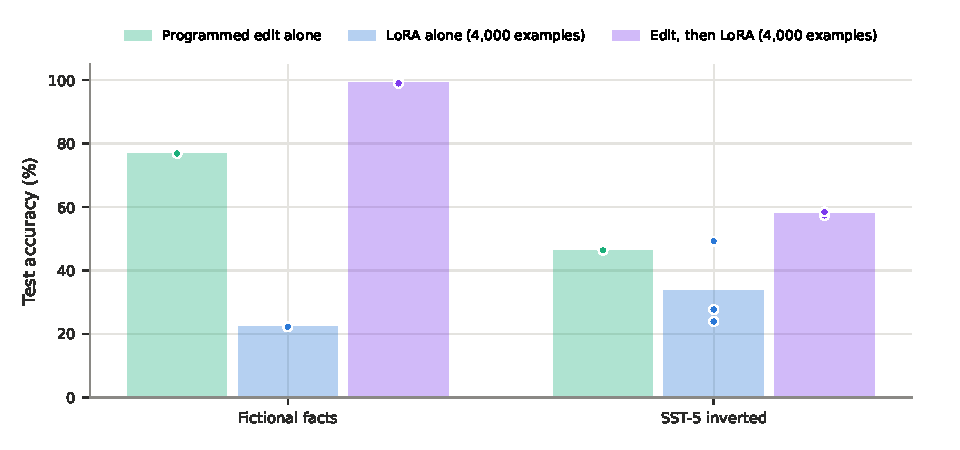
\includegraphics[width=0.8\linewidth]{figures/combination.pdf}
\caption{A programmed edit saves fine-tuning data (Qwen, test accuracy). With 4,000 examples, LoRA from the edit reaches about what LoRA alone reaches with ten times (facts) or three times (SST-5 inverted) the data. Bars are means; dots are individual seeds.}
\label{fig:combination}
\end{figure}

\paragraph{Side effects.} The combined models kept general ability (Table~\ref{tab:combine}).
\begin{itemize}
  \item \textbf{Facts.} MMLU was 58.0--59.6\% over the three seeds (base and edit alone 59.6\%), next-token top-1 45.5\% (base 45.9\%), and accuracy on SST-5 dev 42.6--43.6\% (base 42.3\%).
  \item \textbf{SST-5 inverted.} MMLU was 58.0--58.6\% (edit alone 57.8\%, LoRA alone 55.6\%) and top-1 45.7--45.8\%. Raw perplexity stays high only because of the swap edit's temperature change; one logit rescaling removes it (rescaled NLL 2.79, base 2.77). On SmolLM2, MMLU was 46.6--48.0\% (base 48.8\%) and top-1 46.0\% (base 46.0\%).
\end{itemize}
Every MMLU difference is within its 95\% interval of about $\pm4$ points. \citet{yang2026writing} saw the opposite when they trained LoRA on top of a written patch: the adapter broke neighbouring tasks, as it did when trained from the base model.

\paragraph{Takeaway.} The methods are complements. A programmed edit is cheap and readable but limited. Fine-tuning is general but slow to store new facts and can stall on a confidently wrong start. A programmed edit worked around both of fine-tuning's failure modes we saw, and fine-tuning took both edits well past what programming alone reached. More data fixes both failures too, so what the edit buys is training data: about ten times less on facts and three times less on SST-5 inverted, for about the same final accuracy.

\subsection{Does the programmer matter, and what does programming cost?}
\label{sec:programmer}
\paragraph{The programmer matters when there is something to build.} With the same brief, Fable and Opus did equally well where the fix was a small redirection: 46.2--48.1\% against 45.7\% on SST-5 inverted. Where an edit had to be built, they diverged:
\begin{itemize}
  \item \textbf{Facts.} Fable reached 100\% with bypass circuits; Opus reached 76.9\% through the model's memory.
  \item \textbf{Twin-2K.} Fable reached 45.0\%; Opus reached 31.9\%.
  \item \textbf{SST-5.} Opus found no improving edit at all.
\end{itemize}
Part of the gap is infrastructure: two Opus runs ended early while waiting hours for a GPU. But the direction is what one would expect. Redirection is a small search; building a working circuit is a demanding engineering job.

\paragraph{Cost.} The two methods spend different resources (Appendix Table~\ref{tab:cost}).
\begin{itemize}
  \item \textbf{GPU time.} A programming run scores at most 25,600 examples: minutes of GPU time for short prompts, and about 1.5 T4-hours at most for Twin-2K. LoRA took 29 minutes of T4 time per SST-5 task, 3.6 hours for facts and 5.7 hours for Twin-2K.
  \item \textbf{Programmer API time.} At list prices, a completed programming run cost \$16--\$86, with the two preserve runs higher (\$103 and \$364). An audit cost \$1--\$14.
\end{itemize}
Programming trades GPU hours for frontier-model time. Which is cheaper depends on what each costs you. Combined with fine-tuning, however, a programmed edit cut the GPU time needed on facts by up to tenfold.

\section{What this means}
\label{sec:discussion}

\paragraph{In our runs, programming compiled rather than learned.} We began by asking whether weight-space programming can only redirect what a model knows. It can do more: it can add knowledge. But it adds knowledge in a particular way. In every case where programming beat fine-tuning, the programmer turned the training labels into an explicit object and wrote that object into the weights:
\begin{itemize}
  \item a swapped pair of words (SST-5 inverted);
  \item a table of facts (fictional facts);
  \item a table of answer rates (Twin-2K).
\end{itemize}
Nothing was learned in the sense that fine-tuning learns, by gradually shaping features until they generalise. A compiler can only compile what can be written down. That explains both the strengths and the ceiling. Programming did best where the target is a short rule or a finite table, and worst on SST-5, where it is neither: three independent programmers found three mechanisms and hit the same ceiling.

\paragraph{The knowledge map, and what the probe misses.} Figure~\ref{fig:map} places every method on one chart. For edits that work through the model, the gain roughly tracks the probe's headroom: large where the model holds an unused answer, small where it does not. The probe predicted the redirect regime on both models. It does not predict compiling. Bypass circuits and the Opus memory gain 56--79 points on facts, where the probe finds nothing, and LoRA gains twelve points on Twin-2K, where the probe again finds nothing. A linear probe at one position estimates what a \emph{readout} edit can use. It does not estimate what a programmer who builds new machinery, or a gradient that trains it, can reach. Deciding which regime a task is in therefore still needs judgement. One test is whether the target can be written down from the labels.

\begin{figure}[t]
\centering
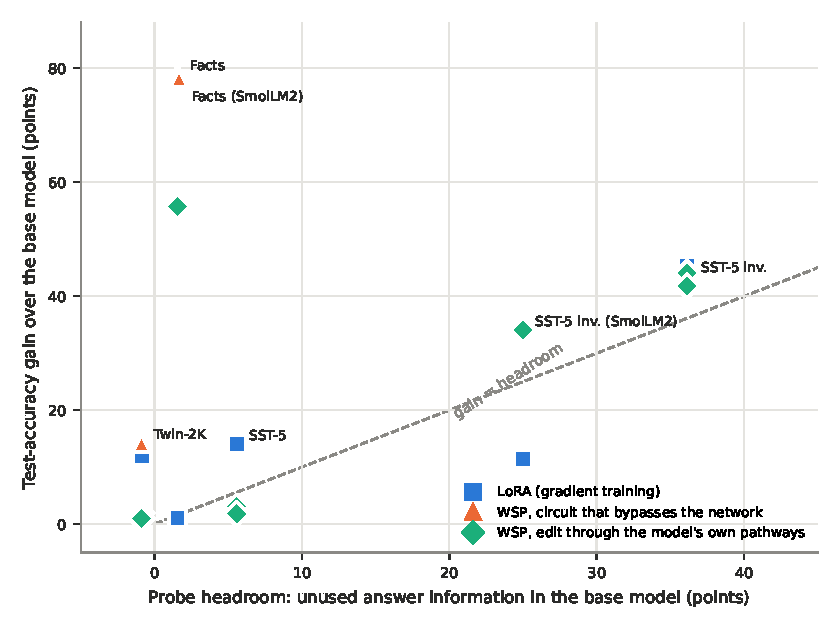
\includegraphics[width=0.75\linewidth]{figures/knowledge_map.pdf}
\caption{The knowledge map: gain over the base model against probe headroom, for every method on both models (test points; preserve runs omitted). Edits through the model's pathways (green) roughly follow the diagonal, recovering about as much as the probe says is unused. Compiled edits (orange, and the Opus facts memory at upper left) sit far above it: they add knowledge the probe says is absent. LoRA (blue) gains on most tasks regardless of headroom, but fails on SST-5 inverted for SmolLM2 and on facts at the default budget.}
\label{fig:map}
\end{figure}

\paragraph{Around or through decides the cost, and the brief decides which.} The finding with the most practical weight concerns side effects. The same information can be written into a model in a way that leaves it intact or one that wrecks it, depending on whether the edit goes around the network or through it.
\begin{itemize}
  \item \textbf{Bypass circuits} are easier to make exact, because the programmer controls every step, so they score highest. But they claim components every input depends on, and their output overwhelms the rest of the computation. On both model families, they left the model at chance on general knowledge.
  \item \textbf{Through edits} have to cooperate with what the network already does, so they are less exact and far less destructive. Fine-tuning is a through edit by construction.
\end{itemize}
The preserve experiment shows the choice belongs mainly to the instruction, not the method. The same programmer that built three destructive facts circuits under the standard brief built a gated, intact edit for Twin-2K when told to preserve the model. It did not manage one for facts, so preservation sometimes costs everything that was gained. This qualifies the conclusion of \citet{yang2026writing} that written edits disturb less: their one published patch was gentler than LoRA, but here the most accurate written edits were far more destructive than LoRA. How gentle an edit is depends on how it is built, not on whether it is written or trained.

\paragraph{How to evaluate an edit.} Two traps appeared, pointing in opposite directions.
\begin{itemize}
  \item \textbf{Target-task accuracy rewards the most damaging edits.}
  \item \textbf{Raw perplexity punishes harmless ones,} because a temperature change multiplies it a hundredfold without changing a single prediction.
\end{itemize}
A minimal protocol that avoided both in our study has four checks:
\begin{itemize}
  \item next-token top-1 accuracy on ordinary text;
  \item a general-knowledge benchmark;
  \item a task unrelated to the edit;
  \item consistency under option reordering.
\end{itemize}
The first three separated bypass from through edits without exception. The last shows whether an edit changed what the model reads or how it reads.

\paragraph{Program first, then fine-tune.} The most useful practical result is that the two methods combine. Fine-tuning failed in two ways that a programmed edit fixed:
\begin{itemize}
  \item \textbf{Slow storage of new facts.} The edit cut the training needed by up to tenfold.
  \item \textbf{A stall on a confidently wrong start.} The edit removed the plateau that stopped two of three seeds on Qwen and all three on SmolLM2. On Qwen, LoRA alone needed three times the data to get past it; we did not try more data on SmolLM2.
\end{itemize}
In return, fine-tuning took each edit far past its own ceiling, and the combined models kept general ability. On SST-5 inverted, the part of the edit that mattered is a two-row swap anyone could write once they know the readout is mirrored; the programmer's contribution was finding it without being told. This suggests a workflow. A programmer inspects the model and writes a small, readable edit for whatever can be redirected or compiled, which takes minutes of GPU time (though \$16--\$86 of programmer API time for a typical run, at list prices), and gradient training does the rest. The edit also documents what the model was missing.

\paragraph{A rule of thumb.} Table~\ref{tab:guide} condenses the results into a choice of tool.

\begin{table}[h]
\centering\small
\begin{tabular}{p{4.4cm}p{3.6cm}p{5.8cm}}
\toprule
If the problem is\ldots & Reach for\ldots & Because\ldots \\
\midrule
The model knows the answer but reads it out wrongly (a flipped label, a misrouted feature) & Weight-space programming, then fine-tuning & Tiny, readable, reproducible edits match fine-tuning, are more reliable, and need fewer labels. Fine-tuning on top adds about ten points (SST-5 inverted). \\
\addlinespace
The model must recall a table and does nothing else & Either; programming is faster on GPU & A compiled lookup matched or beat fine-tuning (facts, Twin-2K). \\
\addlinespace
The model must recall a table \emph{and} keep its other abilities & A programmer told to work through the model's pathways, then fine-tuning & Bypass circuits destroyed general ability; through edits and LoRA did not. An edit plus LoRA reached 99\% with a tenth of LoRA's data and kept general ability. \\
\addlinespace
The model must get better at a mapping it already partly does & Fine-tuning & Programming gained about three points where LoRA gained fourteen, and LoRA still gained nine with only 256 examples (SST-5). \\
\bottomrule
\end{tabular}
\caption{When to program and when to fine-tune, based on our results with 1.5--1.7B models.}
\label{tab:guide}
\end{table}

\paragraph{The programmer matters most when there is something to build.} Two programmer models were equally good at redirection, but the stronger one was much better whenever an edit had to be constructed, and it was also the one that took the destructive route. If programming is compiling, this is what one would expect: the output depends on the engineer, and on the specification the engineer is given. It also means results will change as programmer models improve. Our findings describe what current models do with this budget, not a limit of the method.

\paragraph{A note on simulating people.} Twin-2K adds a finding that matters outside this comparison. Neither fine-tuning nor programming beat the plain per-question answer prior, which ignores the person entirely. The best programmed edit was that prior in circuit form. For a 1.5B model, a person's profile added nothing measurable over knowing what people in general answer. Work that claims to simulate individuals with language models should report this prior as its baseline. A model that beats chance but not the prior is simulating a population.

\section{Limitations}
\label{sec:limitations}

\begin{itemize}
  \item \textbf{Small models, two families.} All results are for 1.5--1.7B instruction-tuned models. Larger models hold more of each task's knowledge, which may move tasks between regimes. For example, a larger model may know enough about people that Twin-2K becomes a redirect task.
  \item \textbf{Run counts are still modest.} Under the standard brief, Fable has:
  \begin{itemize}
    \item on Qwen: three runs each on SST-5, SST-5 inverted and facts, and one on Twin-2K;
    \item on SmolLM2: one run each on SST-5 inverted and facts.
  \end{itemize}
  Opus has one run per Qwen task, and the preserve condition has one run per compile task. Four further Fable runs stopped part-way when a usage limit was reached and are excluded. A second Twin-2K Fable run (\texttt{r4}) finished but broke the no-fitting rule, and is reported separately (Appendix~\ref{app:deviations}).
  \item \textbf{LoRA seeds and tuning.}
  \begin{itemize}
    \item \textbf{Seeds.} SST-5 and SST-5 inverted have three seeds each. Twin-2K, facts and SmolLM2 have one, because those runs take hours.
    \item \textbf{Tuning.} LoRA used one default configuration everywhere except facts, where we searched until it learned.
    \item \textbf{The plateau.} A learning-rate warmup or larger learning rate might help it escape the plateau on SST-5 inverted. We report the failure as a property of the default configuration, not of LoRA in general.
  \end{itemize}
  \item \textbf{Dev use by programmers.} Programmers measured candidates on dev, and some chose among candidates by dev accuracy, or built constants from unlabelled dev activations. The auditors quantified this where possible; on facts it inflated the preserve run's dev gain from about 4 to 6 points. Test numbers, which no programmer saw, are the reliable comparison.
  \item \textbf{Rule boundaries.} Three permissions in the brief are judgement calls:
  \begin{itemize}
    \item label-derived tables, if disclosed;
    \item closed-form solves on weights or activation statistics, such as pseudo-inverses;
    \item one-dimensional grid searches over a scalar.
  \end{itemize}
  Several of the best compile-regime edits rely on the first, so a stricter rule would lower programming's results there.
  \item \textbf{Infrastructure.}
  \begin{itemize}
    \item Two Opus runs ended early because Kaggle GPU sessions were unavailable for hours.
    \item Queued GPU jobs were sometimes cancelled and re-pushed. The ledgers show no pass was charged twice, but one run probably executed a job more than once without charging the duplicate passes.
    \item Some evaluations ran on P100 rather than T4 GPUs. With fp16 inference the effect on letter probabilities is negligible, but the results are not bit-identical.
  \end{itemize}
  \item \textbf{Protocol slips by the orchestrator.} One SST-5 replication (\texttt{r5}) was told another run's result mid-run. Its audit dated its final design to six hours before the message, so we count it as independent. Several remote job outputs were deleted while unsticking the queue; local copies were kept.
\end{itemize}

\section{Conclusion}
Weight-space programming promises a new way to change a model: read the weights, work out the computation, and write the fix directly. We asked when that works and what it costs, holding everything fixed except how much the model already knew, and repeated the key experiments on a second model family.

The answer has four parts.
\begin{itemize}
  \item \textbf{Redirect.} When the model has the knowledge and misreads it, programmers reliably find tiny fixes that match fine-tuning and fail less often.
  \item \textbf{Compile.} When the answer is a table, programmers compile it into the weights and can beat fine-tuning. The most accurate way to do so bypasses the network and leaves the model at chance on general knowledge. An instruction to preserve the model changes the edit the programmer builds, at a cost in accuracy.
  \item \textbf{Learn.} When the improvement has to be learned, fine-tuning wins, even with far fewer labels.
  \item \textbf{Combine.} A programmed edit makes fine-tuning faster and more reliable, and at the same training budget the combination beats both.
\end{itemize}

In our runs, weight-space programming acted as a compiler for rules and tables and a starting point for learning, not a replacement for it. Anyone using or evaluating it should state what must be preserved and measure what an edit does to the rest of the model, with measures a temperature change cannot fake.

\paragraph{Reproducibility.} Code, task builders, the programmer briefs, every programmer's log, edit and final report, all audit reports, the per-run cost accounting and all result files are in a private repository (\url{https://github.com/Puneet-Bajaj-IITM/wsp-vs-lora}), to be made public with the preprint.

\paragraph{Use of AI.} The weight-space programming runs and their audits were carried out by Claude models, as described in Section~\ref{sec:design}. Claude was also used to build the experiment infrastructure and to draft this manuscript. The author reviewed all results and text.


\bibliographystyle{plainnat}
\bibliography{references}

\appendix
\section{The programmer brief}
\label{app:brief}
Each run received the same brief (\texttt{briefs/study.md} in the repository), with task-specific paths and a short task description. Its rules, in brief:
\begin{enumerate}
  \item \textbf{No gradients and no learned fitting.}
  \begin{itemize}
    \item Forbidden: autograd, optimisers, LoRA, and any regression or classifier solver trained against labels (logistic regression, least squares and similar).
    \item Allowed: reading or decomposing weights; simple statistics of forward-pass outputs (means, differences of means, counts, histograms, PCA); and closed-form weight changes the programmer derives.
    \item Allowed with disclosure: a per-item or per-entity table derived from labels and written into the weights.
  \end{itemize}
  \item \textbf{Never read the test split.}
  \item \textbf{Edits are deterministic files} that change existing parameter tensors in place, with constants stored beside them. Architecture changes are not allowed.
  \item \textbf{A budget of 50 forward passes} over train or dev, at most 512 examples each, enforced by a persistent ledger. Running the network outside the ledger is forbidden.
  \item \textbf{Independence}: do not read other runs' folders.
\end{enumerate}
The brief does not mention the study's hypothesis, LoRA results, or other runs' outcomes. SmolLM2 runs received the same brief, with a note that the model description it contains (Qwen's layer count and width) does not apply.

\paragraph{The preserve addendum} (\texttt{briefs/preserve.md}).
\begin{itemize}
  \item The final edit must keep the base model's general abilities; an edit that breaks the model for other uses does not count as a success.
  \item The programmer may score the SST-5 dev set (``preserve'', 1,101 examples) from the same 50-pass budget.
  \item The final edit must score at least 40.0\% on the full preserve set (base: about 42.3\%) and report that number.
  \item Held-out tests of perplexity and general knowledge would also be run, so the edit should leave the model's normal computation intact rather than tune to the preserve set.
\end{itemize}

\section{Audit summary}
\label{app:audits}
Every edit, except the early Twin-2K run \texttt{r1}, was audited by a separate agent. One run (Twin-2K \texttt{r4}) was found to break the brief and is reported in Appendix~\ref{app:deviations}; all others were judged compliant.
\begin{itemize}
  \item \textbf{What the auditor did.} It read every script and edit file, checked the ledger against the jobs actually run, recomputed dev accuracy and NLL from saved log-probabilities, and counted changed weights from the code. For later runs it also read the programmer's full transcript.
  \item \textbf{Verdicts.} All other runs were judged compliant, most ``with notes''. No run read the test split, used gradients, or fitted a classifier to labels. Every reported dev number reproduced exactly, except for one run that saved no per-item outputs; its result was confirmed indirectly.
\end{itemize}
The notes, all disclosed or minor:
\begin{itemize}
  \item \textbf{Label-derived tables in the weights.} Facts \texttt{r1}, \texttt{r2}, \texttt{r4}, \texttt{o1}, \texttt{p1} and SmolLM2 \texttt{f1}; Twin-2K \texttt{r2} and \texttt{o1}. All disclosed.
  \item \textbf{Closed-form solves.} Pseudo-inverses or ridge-regularised matched filters computed from weights, designed codes or label-free activation means: facts \texttt{r4}, \texttt{p1} and SmolLM2 \texttt{f1}; Twin-2K \texttt{p1}; SST-5 \texttt{r5}. The auditors ruled these inside the brief because they are fitted to designed targets, not to labels.
  \item \textbf{Selection on dev.} Several runs chose among candidates, or set a constant, by dev accuracy. The facts preserve run also built some constants from unlabelled dev activations without disclosing it. On the dev questions it had not used, its gain was about 4 points rather than the reported 6.
  \item \textbf{The test template seen but not used.} The facts task builder, which programmers were pointed to, contains the test-split question wording. Three facts runs read that file. Their audits checked that no script used the test wording and that no test-only token appears in their token lists.
  \item \textbf{Local stand-in tests.} One facts run tested its circuit logic on a randomly initialised network of the same shape on the laptop. No study-model weights were loaded.
  \item \textbf{Procedure.} Several runs used their own polling loops, which the brief forbids, and saw other runs' folder names in directory listings, without opening their files.
  \item \textbf{A probable duplicate job.} The facts preserve run probably executed one job more than once through automatically backgrounded push commands. The ledger kept only one set of charges. The run saw only one output, but at least four passes were probably uncharged. We since changed the harness to refuse a second run of a queued or running job, and to stamp every ledger entry with a job identifier.
  \item \textbf{A leaked result.} SST-5 \texttt{r5} was told, while resuming, another run's mechanism and score. The audit dated its final steering configuration to six hours before the message and found nothing after it resembling the leaked idea, so the run counts as independent.
\end{itemize}

\section{Protocol deviations}
\label{app:deviations}
Following standard practice, the main results include only runs that followed the brief. Runs that broke a rule are not dropped; they are reported here with their full numbers.

\paragraph{Twin-2K \texttt{r4} (Fable).} The audit found two problems with this run:
\begin{itemize}
  \item \textbf{A discarded least-squares variant.} One budgeted forward pass applied a read-out fitted by truncated least squares to the label-derived answer-frequency table. It scored 31.3\% on a training sample, lost the run's own selection, and is not in the final edit. Rule~1 forbids such solvers whether or not the result is kept.
  \item \textbf{The final edit is effectively a regression.} Its read-out is written as a label-weighted difference of means multiplied by a fixed matrix, with no solver call. Because that matrix includes the option-token activations themselves, the auditor showed it is mathematically identical to a ridge regression of the label-derived targets on those activations.
\end{itemize}
The programmer disclosed the first point as borderline. It described the matrix as built from generic activations, which the audit found inaccurate.

\paragraph{What the edit is.} It adds rank-1 terms to the key projections of the attention heads in layers 18, 20 and 21 that read the answer options. These heads choose an option by a fixed ``attractiveness'' of its text, which tracks the model's own preference rather than what people answer. The edit tilts that attractiveness toward train answer rates. It changes 172,032 weights, uses 48 of 50 passes, and is a through edit (Table~\ref{tab:deviations}).

\paragraph{Sensitivity.} Including this run would change none of the paper's conclusions:
\begin{itemize}
  \item It is a through edit that keeps the model intact (MMLU 58.8\%, top-1 45.6\%).
  \item It improves Twin-2K by 6.1 points on test, more than any compliant through edit (Opus \texttt{o1}: +1.0; preserve \texttt{p1}: +4.3).
  \item It stays below LoRA (42.8\%) and the answer prior (47.1\%).
\end{itemize}
It would weaken one sentence: under the standard brief, Fable does not always build a bypass circuit for a compile task. It shows what a label-fitted read-out buys through the model's own pathways: about two points more than the compliant preserve edit.

\begin{table}[h]
\centering\small
\resizebox{\linewidth}{!}{\begin{tabular}{llllrrrrrr}
\toprule
Task & Run & Edit type & Test & Dev & Other task & MMLU & Top-1 & Weights & Passes \\
\midrule
Twin-2K & r4 (Fable) & through & 37.0 & 35.6 & 44.1 & 58.8 & 45.6 & 172,032 & 48 \\
\bottomrule
\end{tabular}
}
\caption{Runs excluded from the main comparison for breaking the brief (Qwen, accuracy \%). Columns as in Table~\ref{tab:side}; \emph{Other task} is SST-5 dev (unedited 42.3).}
\label{tab:deviations}
\end{table}

\section{LoRA on the facts task}
\label{app:facts-lora}
Table~\ref{tab:facts-lora} lists every LoRA configuration we tried on facts and facts-60.
\begin{table}[h]
\centering\small
\begin{tabular}{llrrr}
\toprule
Task & Config & Epochs & Dev & Test \\
\midrule
facts & lr $10^{-4}$, 4,000 ex. (default) & 1.5 & 21.4 & 22.2 \\
facts & lr $10^{-3}$, 12,000 ex. & 4.4 & 21.3 & 18.9 \\
facts & lr $3\times10^{-4}$, 12,000 ex. & 4.4 & 19.8 & 21.1 \\
facts & lr $10^{-4}$, 40,500 ex. & 15 & 99.2 & 98.8 \\
facts-60 & lr $10^{-4}$, 8,000 ex. & 15 & 98.3 & 96.7 \\
facts-60 & lr $3\times10^{-4}$, 8,000 ex. & 15 & 22.8 & 20.0 \\
\bottomrule
\end{tabular}
\caption{LoRA on the facts tasks (accuracy \%). Dev and test use question wordings not seen in training.}
\label{tab:facts-lora}
\end{table}

\section{What each edit changed, and what it cost}
\label{app:cost}
\begin{table}[h]
\centering\scriptsize
\resizebox{\linewidth}{!}{\begin{tabular}{llrrrrp{5.4cm}}
\toprule
Task & Run & Weights changed & Fraction & Passes & API cost & Mechanism \\
\midrule
SST-5 & r1 (Fable) & 2,338,393 & 0.1515\% & 49 & \$49 & L19 neutral-detector neurons, L21 query re-mapping, temperature \\
SST-5 & r4 (Fable) & 6,144 & 0.0004\% & 47 & \$20 & one repurposed layer-19 MLP neuron adding a constant class-prior shift (less very-negative, more neutral) + temperature \\
SST-5 & r5 (Fable) & 2,304 & 0.0001\% & 44 & \$86 & value-bias steering at layers 17/19/21 from 'very' toward plain class centroids + temperature \\
SST-5 & o1 (Opus) & 0 & -- & 19 & \$35 & no edit beat base (run cut short by Kaggle queueing) \\
SST-5 inverted & r1 (Fable) & 791,040 & 0.0512\% & 44 & \$16 & swap negative/positive embeddings, rank-1 intensity steer, temperature \\
SST-5 inverted & r2 (Fable) & 4,608 & 0.0003\% & 24 & \$20 & swap negative/positive embeddings, temperature \\
SST-5 inverted & r3 (Fable) & 5,632 & 0.0004\% & 18 & \$25 & swap negative/positive embeddings, neutral steer, temperature \\
SST-5 inverted & o1 (Opus) & 6,144 & 0.0004\% & 29 & \$31 & swap negative/positive embeddings, neutral mix, temperature \\
Twin-2K & r1 (Fable*) & 12,288 & 0.0008\% & 20 & \$85 & option-word embedding remaps, temperature \\
Twin-2K & r2 (Fable) & 32,258,170 & 2.0896\% & 20 & \$76 & hand-built layer-0-2 circuit computing the train answer prior \\
Twin-2K & o1 (Opus) & 6,144 & 0.0004\% & 24 & \$28 & one layer-20 neuron carrying per-option-text offsets, temperature \\
Twin-2K & p1 (Fable, preserve) & 785,389 & 0.0509\% & 27 & \$103 & gated rank-3 q\_proj update on layer-21 selector heads 8-11, steering attention toward options respondents choose (3 answer styles) \\
Fictional facts & r1 (Fable) & 8,152,867 & 0.5281\% & 10 & \$32 & hand-built layer-0/1 lookup circuit over name tokens \\
Fictional facts & r2 (Fable) & 3,705,795 & 0.2401\% & 6 & \$45 & hand-built layer-0/1 lookup circuit over name tokens \\
Fictional facts & r4 (Fable) & 6,182,912 & 0.4005\% & 17 & \$39 & hand-built layer-0/1 lookup circuit: name-gather heads, letter-bind head, 900 fact neurons, layer-1 readout \\
Fictional facts & o1 (Opus) & 4,147,200 & 0.2687\% & 44 & \$56 & 900 layer-8 MLP neurons keyed on name tokens, writing value vectors \\
Fictional facts & p1 (Fable, preserve) & 3,069,184 & 0.1988\% & 49 & \$364 & flag-gated person memory (300 MLP-17 detectors writing private codes, 30 MLP-20 value writers) + attention-16 constant; fails preserve (0.381) \\
\bottomrule
\end{tabular}
}
\caption{Every Qwen edit: weights changed out of 1,543,714,304, budgeted forward passes used (at most 50 passes of 512 examples), and the programmer's API cost at list prices, computed from its transcript (input, output and cache tokens). SmolLM2 runs: SST-5 inverted 22,528 weights, 39 passes, \$18; facts 5.57M weights, 4 passes, \$21.}
\label{tab:cost}
\end{table}

\paragraph{Tokens.} Table~\ref{tab:tokens} totals the tokens behind these costs, including the runs that stopped part-way. Almost all of the volume is the agents re-reading their own growing context from the prompt cache. Uncached input is negligible (under 15,000 tokens per model), and generated output totals about 7.2M tokens across all runs. The totals exclude the orchestrating session and the agent that built the experiment infrastructure.
\begin{table}[h]
\centering\small
\begin{tabular}{llrrrrr}
\toprule
Role & Model & Runs & Output (M) & Cache read (M) & Cache write (M) & Cost \\
\midrule
Programmers & Fable 5.1 & 1 & 0.33 & 26.6 & 3.3 & \$85 \\
Programmers & Fable 5.2 & 19 & 5.29 & 470.5 & 81.2 & \$1,118 \\
Programmers & Opus 5.5 & 4 & 0.85 & 208.8 & 18.3 & \$150 \\
Auditors & Opus 5.5 & 18 & 0.72 & 111.8 & 5.1 & \$62 \\
\bottomrule
\end{tabular}

\caption{API tokens (millions) and cost at list prices by role and model, over all programmer runs (including the four stopped runs and the excluded Twin-2K \texttt{r4}) and all audits.}
\label{tab:tokens}
\end{table}


\end{document}
